%%%%%%%%%%%%%%%%%%%%%%%%%%%%%%%%%%%%%%%%%%%%%%%%%%%%%%%%%%%%%%%%%%%%%%%%%%%%%%%%%%%%%%%%%
\exo \textbf{Loi de Wien}

\vspace{0.3cm}

\textbf{Document $1$}

\begin{figure}[h]
\begin{center}
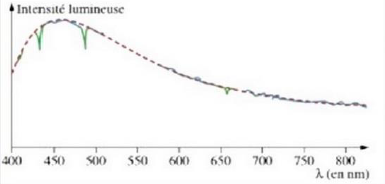
\includegraphics[width=0.5\columnwidth]{images/Exo1_Profil_Spectral_Etoile_Riga}
\end{center}
\caption{\label{fig:Profil_Spectral_Etoile_Riga}
Profil spectral de l'étoile de Riga}\end{figure}

\vspace{0.3cm}

\textbf{Document $2$}

\begin{figure}[h]
\begin{center}
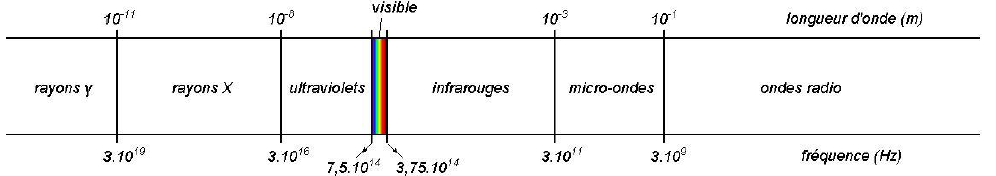
\includegraphics[width=\columnwidth]{images/Exo1_Spectre_Rayonnements_EM}
\end{center}
\caption{\label{fig:Spectre_Rayonnements_EM}
Spectre des rayonnements électromagnétiques}\end{figure}

\vspace{0.3cm}

\textbf{Document $3$ : loi de Wien}

\vspace{0.3cm}

La loi de Wien s'applique aux sources chaudes (aussi appelées corps noirs) et permet de relier la température $T$ d'une source chaude à la longueur d'onde de l'intensité maximale $\lambda_{max}$. La loi de Wien peut s'écrire sous forme de la formule suivante:

$$T = \frac{2.89 \times 10^{-3}}{\lambda_{max}}$$

avec $T$ en Kelvin ($\kelvin$), $\lambda_{max}$ en mètre ($\meter$), et la constante en Kelvin.mètre ($\kelvin.\meter$).

\vspace{0.3cm}

Le lien entre degré Celsius et Kelvin est donné par la relation: $\Theta(\celsius) = T - 273.15$.

\vspace{0.3cm}

\textbf{Document $4$ :} quelques détails sur les lampes halogènes:

\vspace{0.3cm}

En faisant passer un courant électrique dans le filament d'une ampoule, la température du filament s'élève: la couleur de la lumière émise par cette ampoule dépend alors de la température du filament.\newline
Les lampes halogènes contiennent un filament au tungstène chauffé à $3200$ \kelvin : une température plus élevée que dans les ampoules à filament classique. Ainsi la lumière fournie par une ampoule halogène est plus blanche et donne un meilleur rendu des couleurs, mais émet aussi des UV. C'est pourquoi une ampoule
halogène a toujours un verre de protection qui absorbe les UV.\newline
L'inconvénient des sources thermiques est qu'une grosse partie de l'énergie électrique n'est pas utilisée
pour produire de la lumière, mais de la chaleur.

%\vspace{0.3cm}

\newpage

A l'aide des documents ci-dessus et de vos connaissances, répondre aux questions suivantes:

\begin{enumerate}
\item Compléter le tableau ci-dessous (à reproduire sur la copie) en justifiant les résultats de la première ligne.

\begin{center}
\begin{tabular}{|c|c|c|c|}
\hline
Objet & $\lambda_{max}$ & $\Theta$ & Domaine du spectre \\
\hline
Corps humain &      &       &       \\
\hline
Etoile Riga &       &       &       \\
\hline
Lampe d'ambiance rouge  &       &       &   \\
\hline
Lampe halogène  &       &       &       \\
\hline
\end{tabular}
\end{center}

\item Donner la définition des grandeurs intervenant dans la loi de Wien.

\item On peut trouver la loi de Wien avec la formule $\lambda_{max} T = 2.89 \times 10^{6}$. Expliquer. Quelle est alors l'unité de $\lambda_{max}$ et de $2.89 \times 10^{6}$ ?

\item \begin{enumerate}[label=(\alph*)]
\item En utilisant la loi de Wien, expliquer comment évolue la longueur d'onde du maximum d'intensité en fonction de la température du corps chaud.
\item Justifier alors la phrase "la lumière fournie par une ampoule halogène est plus blanche […], mais émet
des UV" du document $4$.
\end{enumerate}

\end{enumerate}

\vspace{0.3cm}

%%%%%%%%%%%%%%%%%%%%%%%%%%%%%%%%%%%%%%%%%%%%%%%%%%%%%%%%%%%%%%%%%%%%%%%%%%%%%%%%%%%%%%%%%
\exo \textbf{Solutions aqueuses}

\vspace{0.3cm}

\textit{Données: }$N_{A} = 6,02.10^{23}\text{ }\mole^{-1}$; $M(C) = 12,0\text{ }\gram.\mole^{-1}$; $M(H) = 1,00\text{ }\gram.\mole^{-1}$; $M(N) = 14,0\text{ }\gram.\mole^{-1}$; $M(O) = 16,0\text{ }\gram.\mole^{-1}$; $M(Cu)=63,5\text{ }\gram.\mole^{-1}$; $M(S)=32,1\text{ }\gram.\mole^{-1}$

\vspace{0.3cm}

A température ordinaire, le sulfate de cuivre pentahydraté, est un solide soluble dans l'eau. Sa formule brute est (\chemform{CuSO_{4},5H_{2}O}).\newline
On se propose de préparer $V = 100\text{ }\milli\liter$ d'une solution de sulfate de cuivre pentahydraté dont la concentration molaire en sulfate de cuivre pentahydraté est $C = 0,10\text{ }\mole.\liter^{-1}$.

\begin{enumerate}
\item Préciser quel est le soluté et quel est le solvant dans la solution à préparer.

\item Quelle est la quantité de matière n en sulfate de cuivre pentahydraté contenue dans $V = 100\text{ }\milli\liter$ de solution à préparer ?

\item Quelle est la masse $m$ de sulfate de cuivre pentahydraté à prélever pour préparer ces $100\text{ }\milli\liter$ de solution ?

\item Rédiger le protocole expérimental permettant de préparer cette solution.\newline
A partir de cette solution on souhaite préparer $V'=100\text{ }\milli\liter$ de solution de sulfate de cuivre pentahydraté de
concentration $C' = 0,010\text{ }\mole.\liter^{-1}$.

\item Comment s'appelle cette opération ?

\item Calculer le volume $V_{p}$ de solution mère à prélever pour préparer cette solution ?

\item Rédiger le protocole expérimental permettant de préparer cette solution.\newline
Faire une série de schémas résumant les différentes étapes du protocole.

\item On souhaite préparer une solution $S''$ de concentration $0,020\text{ }\mole.\liter^{-1}$. A partir de quelle solution peut-on fabriquer $S''$ ? Justifier votre réponse.

\end{enumerate}

%\vspace{0.3cm}

\newpage

%%%%%%%%%%%%%%%%%%%%%%%%%%%%%%%%%%%%%%%%%%%%%%%%%%%%%%%%%%%%%%%%%%%%%%%%%%%%%%%%%%%%%%%%%
\exo \textbf{Lampes}

\vspace{0.3cm}


\textbf{Document $1$ :} les lampes à vapeur de néon.

\vspace{0.3cm}

On appelle par abus de langage « tube néon » les tubes fluorescents allongés vendus dans le
commerce. Ces tubes contiennent, en général, de la vapeur de mercure sous faible pression. Les véritables tubes au néon produisent une lumière rouge, utilisée principalement dans des enseignes lumineuses. Lorsque la lampe est mise sous tension, des électrons circulent dans le gaz entre deux électrodes. Les électrons cèdent alors de l'énergie
aux atomes qui s'excitent, puis se désexcitent en émettant de la lumière.

\vspace{0.3cm}

\begin{minipage}[c]{.46\linewidth}
\textbf{Document $2$ : niveaux d'énergie de l'atome de Néon}
%\vspace{0.3cm}
\begin{center}
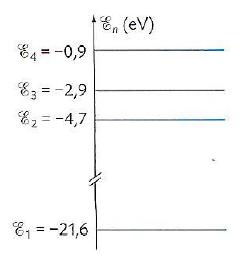
\includegraphics[width=0.5\columnwidth]{images/Exo3_Diagramme_Niveaux_Energie_Neon}
\end{center}
\end{minipage}
\begin{minipage}[c]{.46\linewidth}
\textbf{Document $3$ : niveaux d'énergie de l'atome de Mercure}
%\vspace{0.3cm}
\begin{center}
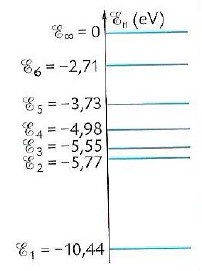
\includegraphics[width=0.4\columnwidth]{images/Exo3_Diagramme_Niveaux_Energie_Mercure}
\end{center}
\end{minipage}

\vspace{0.3cm}

\textbf{Document $4$}

\begin{figure}[h]
\begin{center}
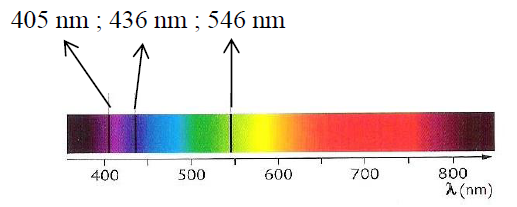
\includegraphics[width=0.75\columnwidth]{images/Exo3_Spectre_Absorption_Mercure}
\end{center}
\caption{\label{fig:Spectre_Absorption_Mercure}
Spectre simplifié d'absorption du Mercure}
\end{figure}

\vspace{0.3cm}

\textbf{Document $5$ :} données

\vspace{0.3cm}

$$h=6,63 . 10^{-34}\text{ }\joule.\second\text{; }1\text{ }\electronvolt = 1,60 . 10^{-19}\text{ } \joule\text{; }c = 3,00\text{ }.\text{ }10^{8}\text{ } \meter.\second^{-1}$$

\vspace{0.3cm}

Parmi les radiations émises par le tube au néon, l'une d'elles possède une longueur d'onde dans le vide $\lambda = 632,8\text{ }\nano\meter$.

\begin{enumerate}
\item \begin{enumerate}[label=(\alph*)]
\item Calculer, en joule puis en électronvolt, l'énergie du photon associé à cette radiation.
\item Cette énergie est-elle gagnée ou perdue par l'atome de néon qui émet cette radiation ?
\item Schématiser, par une flèche sur un diagramme d'énergie, la transition correspondante.
\end{enumerate}
\item Un atome de néon est dans l'état d'énergie $E_{e}$.
\begin{enumerate}[label=(\alph*)]
\item Peut-il changer d'état sous l'effet d'une radiation lumineuse d'énergie $E = 2,9\text{ }\electronvolt$ ? $E = 1,8\text{ }\electronvolt$ ? $E = 16,9\text{ }\electronvolt$ ?
\item Comment ce changement d'état se traduit-il sur le spectre de l'atome ?
\end{enumerate}
\item A l'aide du document $3$, associer une transition énergétique à chaque raie noire du spectre du document $4$.
\end{enumerate}.

\newpage

NB : on considèrera comme égaux des résultats dont l'écart (pour un même nombre de chiffres significatifs) est inférieur ou égal à $0,01\text{ }\electronvolt$.

\vspace{0.3cm}

%%%%%%%%%%%%%%%%%%%%%%%%%%%%%%%%%%%%%%%%%%%%%%%%%%%%%%%%%%%%%%%%%%%%%%%%%%%%%%%%%%%%%%%%%
\exo \textbf{Synthèse du paracétamol}

\vspace{0.3cm}

Le paracétamol est un médicament qui se rapproche de l'aspirine par ses propriétés analgésiques et antipyrétiques. On l'obtient par réaction entre le paraaminophénol et l'anhydride éthanoïque. L'autre produit
de la réaction est l'acide éthanoïque.

\begin{figure}[h]
\begin{center}
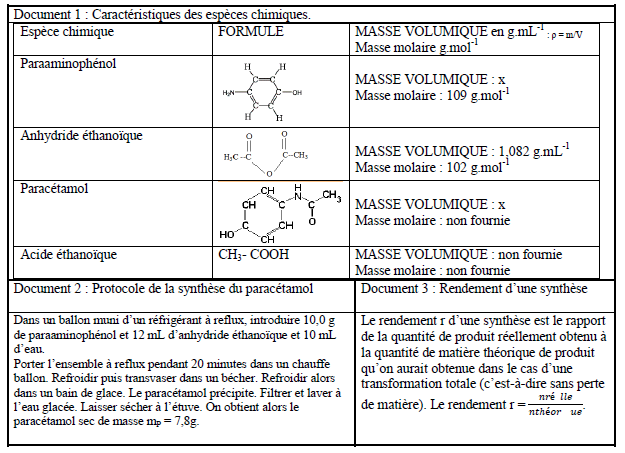
\includegraphics[width=\columnwidth]{images/Exo4_Document_123}
\end{center}
%\caption{\label{fig:Spectre_Absorption_Mercure}Spectre simplifié d'absorption du Mercure}
\end{figure}

\vspace{0.3cm}

\textbf{Document $4$ :} masse molaire des atomes.

$$M(H) = 1,0\text{ }\gram.\mole^{-1}\text{; }M(C)=12,0\text{ }\gram.\mole^{-1}\text{; }M(N)=14,0\text{ }\gram.\mole^{-1}\text{; }M(O)=16,0\text{ }\gram.\mole^{-1}$$

\vspace{0.3cm}

\textbf{Généralités sur le protocole de synthèse}

\begin{enumerate}
\item Légender le schéma expérimental ci-dessous.
\item Pour quelle raison doit-on refroidir le mélange obtenu à la fin de la synthèse ?
\end{enumerate}

\begin{figure}[h]
\begin{center}
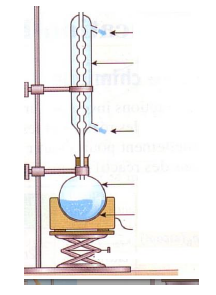
\includegraphics[width=0.25\columnwidth]{images/Exo4_Schema_Experimental}
\caption{\label{fig:Schema_Exp}Schéma expérimental à compléter}
\end{center}
\end{figure}

%\vspace{0.3cm}

\newpage

\textbf{Bilan quantitatif de la synthèse}

\begin{enumerate}
\item L'équation de la réaction de synthèse est:

\begin{chemmath}
C_{6}H_{7}ON + 2C_{4}H_{6}O_{3} + H_{2}O \longrightarrow C_{8}H_{9}O_{2}N + 3C_{2}H_{4}O_{2}
\end{chemmath}

Relier les formules brutes de cette équation aux noms des réactifs est des produits de cette synthèse.

\item Calculer les quantités de matières initiales des réactifs (l'eau est supposée en excès : on ne calculera
donc pas sa quantité de matière ; elle sera notée en excès dans le tableau d'avancement).

\item Etablir le tableau d'avancement de la réaction.

\item Déterminer l'avancement maximal xmax. Le mélange initial est-il dans les proportions
stœchiométriques ? Justifier.

\item En déduire la quantité de matière $n_{P}$ (théorique) de paracétamol qu'on obtiendrait si la réaction était totale.

\item Calculer la quantité de matière $n_{P}$ (réelle) de paracétamol réellement obtenu à l'issue du protocole.

\item Quel est le rendement de la synthèse du paracétamol ?

\end{enumerate}

\vspace{0.3cm}

%%%%%%%%%%%%%%%%%%%%%%%%%%%%%%%%%%%%%%%%%%%%%%%%%%%%%%%%%%%%%%%%%%%%%%%%%%%%%%%%%%%%%%%%%
\exo \textbf{A propos du dioxyde de soufre}

\vspace{0.3cm}

\textbf{Document $1$}

\vspace{0.3cm}

Le dioxyde de soufre de formule \chemform{SO_{2}} est un polluant atmosphérique. En particulier les moteurs des véhicules à essence réalisent la combustion du soufre présent dans l'essence.
De nombreuses réactions peuvent conduire à la formation du dioxyde de soufre. L'une des plus
courantes est la combustion du sulfure d'hydrogène \chemform{H_{2}S} qui produit également de l'eau.
Une fois dans l'atmosphère, le dioxyde de soufre réagit avec l'eau pour former l'acide sulfurique de formule \chemform{H_{2}SO_{4}}. Cette molécule se dissout dans l'eau pour former des ions sulfates \chemform{SO_{4}^{2-}} et des ions \chemform{H^{+}}.\newline
\textbf{L'augmentation de la concentration en ions \chemform{H^{+}} dans l'eau provoque un abaissement du \chemform{pH} et la formation de pluies acides.}

\vspace{0.3cm}

\textbf{Document $2$ : réactions acide/base}

\vspace{0.3cm}

Les ions \chemform{HO^{-}} peuvent réagir avec les ions \chemform{H^{+}} pour former de l'eau. La réaction est totale et libère de l'énergie sous forme de chaleur. On utilise souvent cette réaction pour déterminer la concentration en ions H+ dans une solution: au moment où les réactifs ont été introduits dans les proportions stœchiométriques, il n'y a plus d'ions \chemform{H^{+}} ni d'ions \chemform{HO^{-}} dans la solution, ce qui permet de déterminer la concentration recherchée.

%\vspace{0.3cm}

\newpage

\textbf{Document $3$ : le BBT, un indicateur coloré}

\vspace{0.3cm}

Le BBT est indicateur coloré acido-basique. Il colore une solution en jaune si la solution est acide, il la colore en bleu si elle est basique. Lorsque la solution est neutre, il donne une couleur intermédiaire verte. Dans ce dernier cas, la concentration en ions \chemform{H^{+}} est de $1,0 . 10^{-7}\text{ }\mole.\liter^{-1}$.

\vspace{0.3cm}

\textbf{Document $4$ : réaction de combustion}

\vspace{0.3cm}

Une combustion est une réaction d'oxydoréduction exothermique au cours de laquelle un combustible réagit avec un comburant. Le comburant le plus courant étant le dioxygène de l'air. Pour se produire, une telle réaction nécessite une énergie d'activation souvent apportée par une
source de chaleur. La chaleur produite par la réaction entretient le mécanisme de combustion.

\vspace{0.3cm}

\textbf{Document $5$ : données de quelques éléments}

%\vspace{0.3cm}

\begin{center}
\begin{tabular}{|c|c|c|c|}
\hline
Elément & Numéro atomique & Masse molaire ($\gram.\mole^{-1}$) & Electronégativité \\
\hline
Hydrogène & $1$ & $1,0$ & $2,2$ \\
\hline
Oxygène & $8$ & $16,0$ & $3,44$ \\
\hline
Soufre & $16$ & $32,1$ & $2,78$ \\
\hline
\end{tabular}
\end{center}

\begin{enumerate}
\item Déterminer la formule de Lewis du sulfure d'hydrogène.
\item En déduire la géométrie de la molécule.
\item Cette molécule est-elle polaire ?
\item Cette molécule est-elle soluble dans l'eau ? Justifier.
\item Proposer une équation pour la réaction de combustion du soufre et pour la combustion du sulfure d'hydrogène.
\item Ecrire l'équation de la dissolution de l'acide sulfurique dans l'eau.
\item Nommer et décrire les $3$ étapes du processus de dissolution.

\vspace{0.3cm}

Au laboratoire, on dispose d'une solution d'acide sulfurique à $13\text{ }\mole.\liter^{-1}$.

\item Déterminer la concentration en ions \chemform{H^{+}} et en ions \chemform{SO_{4}^{2-}} dans la solution.

\vspace{0.3cm}

On prélève $10\text{ }\milli\liter$ de cette solution que l'on introduit dans une fiole jaugée de $1\text{ }\liter$, puis on complète avec de l'eau distillée.

\item Comment s'appelle cette opération ?

\item Décrire les étapes de cette préparation par une série de schémas légendés.

\item Déterminer la nouvelle concentration en ions \chemform{H^{+}} et \chemform{SO_{4}^{2-}}.

\vspace{0.3cm}

Pour vérifier l'affirmation selon laquelle le dioxyde de soufre se dissous dans l'eau et abaisse son \chemform{pH}, on réalise la combustion du soufre et l'on récupère le gaz formé pour le faire barboter dans $50\text{ }\milli\liter$ d'eau distillée. On suppose que la totalité du gaz formé se dissout dans l'eau.\newline
On verse alors de la soude (\chemform{Na^{+}+ HO^{-}}) dans le bécher après y avoir ajouté quelques gouttes de BBT. Il faut verser $15\text{ }\milli\liter$ de soude de concentration $C = 2,0 . 10^{-1}\text{ }\mole.\liter^{-1}$ pour voir la solution virer au vert.

\item En vous appuyant sur les documents, montrer que l'affirmation en gras du document $1$ est vérifiée et déterminer la concentration en ions \chemform{H^{+}} dans la solution.

\end{enumerate}

%\vspace{0.3cm}

\newpage

%%%%%%%%%%%%%%%%%%%%%%%%%%%%%%%%%%%%%%%%%%%%%%%%%%%%%%%%%%%%%%%%%%%%%%%%%%%%%%%%%%%%%%%%%
\exo \textbf{Alcanes et alcools}

\vspace{0.3cm}

\textbf{Partie A}

\begin{enumerate}

\item Dans le tableau ci-dessous, identifier et nommer (uniquement) les alcanes et les alcools. Présenter les résultats dans un tableau (à réaliser sur la copie) en reproduisant les formules
sélectionnées.

\begin{figure}[h]
\begin{center}
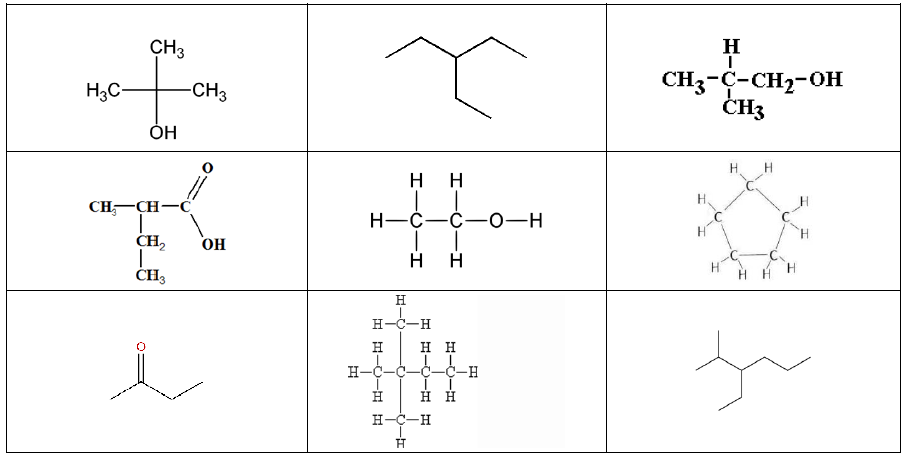
\includegraphics[width=\columnwidth]{images/Exo6_Alcanes_Alcools}
\end{center}
%\caption{\label{fig:Logo Objectif Prépas}
\end{figure}

\item Trouver les trois alcools isomères du butan-1-ol. Donner leur formule semi-développée, et leur nom.

\end{enumerate}

\vspace{0.3cm}

\textbf{Partie B}

\vspace{0.3cm}

On réalise la distillation fractionnée d'un mélange comprenant $4$ espèces chimiques. Au cours de cette distillation, un premier distillat (n°$1$) est récupéré à une température d'ébullition $\theta_{1} = 60\text{ }\celsius$. Un second distillat (n°$2$) apparaît à une température d'ébullition de $80\text{ }\celsius$. Enfin, un troisième distillat (n°$3$) est récupéré pour une température d'ébullition de $116\text{ }\celsius$. On stoppe le chauffage à $120\text{ }\celsius$.

\begin{enumerate}

\item Légender le schéma d'une distillation fractionnée en annexe $3$.

\item On propose, dans le tableau fourni en annexe $2$, les espèces susceptibles de se trouver dans le mélange initial.\newline
A l'aide des documents ci-après, dire dans chaque cas si cette espèce est présente dans le mélange initial, et si oui, quelle est sa température d'ébullition. Pour les espèces présentes dans le mélange, donner leur formule semi-développée et préciser si elles se trouvent dans le distillat numéro $1$, $2$ ou $3$, ou dans le ballon en fin de distillation.

\end{enumerate}

%\vspace{0.3cm}

\newpage

\textbf{Annexe $1$ : données relatives aux changements d'états des alcanes et des alcools}

\begin{figure}[h]
\begin{center}
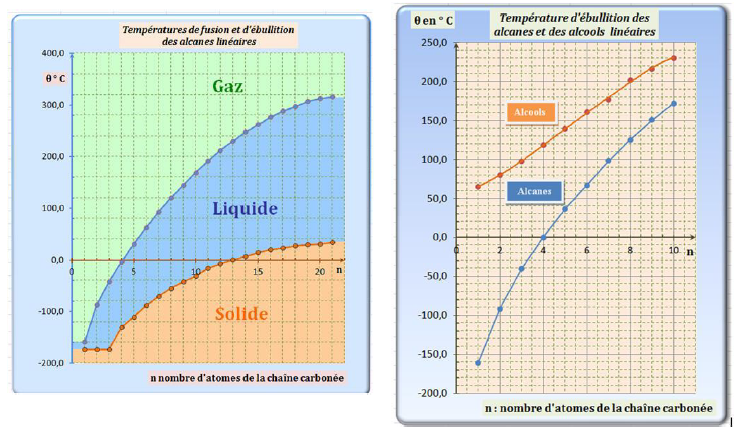
\includegraphics[width=0.5\columnwidth]{images/Exo6_Alcanes_Alcools_Donnees}
\end{center}
%\caption{\label{fig:Logo Objectif Prépas}
\end{figure}

Un alcane ramifié possède une température de changement d'état plus faible que l'alcane linéaire qui possède le même nombre d'atomes de carbone.\newline
De même, un alcool ramifié possède une température de changement d'état plus faible que l'alcool linéaire qui possède le même nombre d'atomes de carbone.

\vspace{0.3cm}

%\newpage

\textbf{Annexe $2$}

\begin{center}
\begin{tabular}{|c|c|c|c|c|}
\hline
Nom & Présente dans le mél. (oui/non) & $\theta$ d'ébull. & Si oui, où ? & Si oui, form. semi-dév. \\
\hline
2-méthylpentane     &   &   &   &   \\
\hline
méthanol            &   &   &   &   \\
\hline
hexan-2-ol          &   &   &   &   \\
\hline
2,3-diméthylhexane  &   &   &   &   \\
\hline
propan-2-ol         &   &   &   &   \\
\hline
méthylbutane        &   &   &   &   \\
\hline
éthanol             &   &   &   &   \\
\hline
\end{tabular}
\end{center}

\vspace{0.3cm}

\textbf{Annexe $3$}

\begin{figure}[h]
\begin{center}
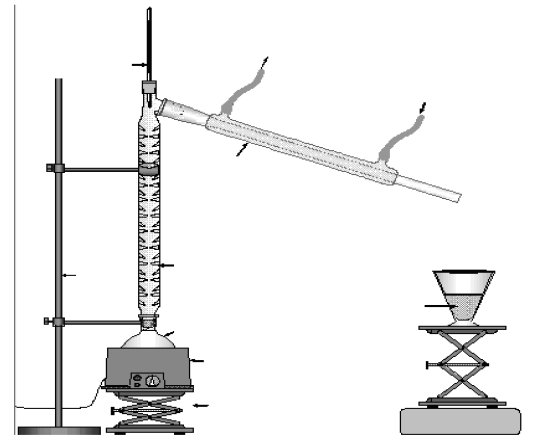
\includegraphics[width=0.5\columnwidth]{images/Exo6_Alcanes_Alcools_Annexe3}
\end{center}
%\caption{\label{fig:Logo Objectif Prépas}
\end{figure}

%\vspace{0.3cm}

\newpage

%%%%%%%%%%%%%%%%%%%%%%%%%%%%%%%%%%%%%%%%%%%%%%%%%%%%%%%%%%%%%%%%%%%%%%%%%%%%%%%%%%%%%%%%%
\exo \textbf{Niveaux d'énergies de l'atome}

\vspace{0.3cm}

\textbf{Document $1$}

\vspace{0.3cm}

Les niveaux d'énergie de l'atome dépendent de la répartition des électrons dans les différentes couches électroniques. Suite à une excitation, les électrons d'un atome peuvent passer d'un niveau d'énergie à un autre
réalisant ainsi une transition énergétique. Ces transitions donnent une raie d'émission. Parfois, les longueurs d'ondes des raies émises sont très proches alors qu'elles appartiennent à deux éléments chimiques différents.

\vspace{0.3cm}

\textbf{Document $2$ : niveaux d'énergie des atomes de quelques éléments chimiques}

%\vspace{0.3cm}

\begin{figure}[h]
\begin{center}
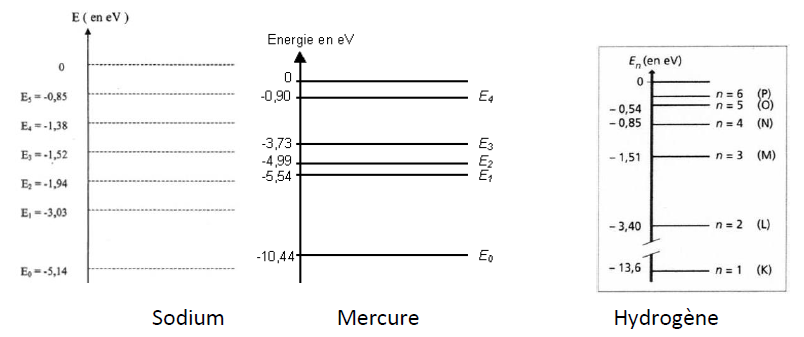
\includegraphics[width=0.75\columnwidth]{images/Exo7_Niveaux_Energie_Atomes}
\end{center}
%\caption{\label{fig:Logo Objectif Prépas}
\end{figure}

\vspace{0.3cm}

Par la méthode de votre choix, rédiger un raisonnement permettant de justifier à quel élément appartient le spectre
ci-dessous. Des calculs sont attendus.

\begin{figure}[h]
\begin{center}
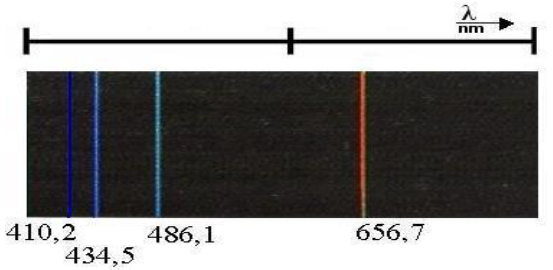
\includegraphics[width=0.5\columnwidth]{images/Exo7_Spectre_Raies_Emission}
\end{center}
%\caption{\label{fig:Logo Objectif Prépas}
\end{figure}

\vspace{0.3cm}

\textit{On attend un raisonnement bien rédigé ! Toute trace (schéma, loi énoncée, calculs...) d'une tentative de raisonnement ou de résolution sera valorisée par des
points (même si le résultat est faux ou incomplet) !}

\vspace{0.3cm}

\underline{Données}

\vspace{0.3cm}

\noindent Constante de Planck: $h = 6,63 . 10^{-34}\text{ }\joule.\second$\newline
Electronvolt: $1\text{ }\electronvolt = 1,60 . 10^{-19}\text{ }\joule$\newline
Vitesse de la lumière dans le vide: $c = 3,00 . 10^{8}\text{ }\meter.\second^{-1}$

%\vspace{0.3cm}

\newpage

%%%%%%%%%%%%%%%%%%%%%%%%%%%%%%%%%%%%%%%%%%%%%%%%%%%%%%%%%%%%%%%%%%%%%%%%%%%%%%%%%%%%%%%%%
\exo \textbf{Energie mécanique}

\vspace{0.3cm}

\begin{minipage}[c]{.46\linewidth}
Pour mesurer sa "force" à la fête foraine, Stéphanie lance un gros palet assimilable à un point matériel de masse $m$. Elle le lance avec une vitesse $V_{0}$ d'un point $A$ d'un plan incliné d'un angle $\alpha$ par
rapport à l'horizontale vers un point $B$ situé plus haut de telle sorte que le palet glisse sur le plan incliné de $A$ vers $B$.
\end{minipage}
\begin{minipage}[c]{.46\linewidth}
\begin{center}
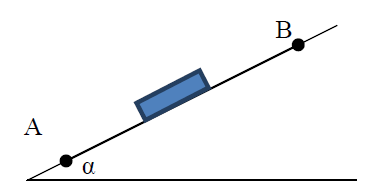
\includegraphics[width=0.75\columnwidth]{images/Exo8_Energie_Mecanique}
\end{center}
\end{minipage}

\begin{enumerate}
\item On néglige les frottements sur le plan. \begin{enumerate}[label=(\alph*)]
\item Dans ce cas, le système est-il en chute libre ?
\item Donner l'expression de l'énergie cinétique $E_{c}(A)$, de l'énergie potentielle de pesanteur du système, puis celle de son énergie mécanique $E_{m}(A)$ en $A$. Donner les unités de chaque grandeur.
\item Même question lorsque le système est en $B$.
\item Si l'énergie mécanique du système se conserve, quelle relation existe-t-il entre $E_{m}(A)$ et $E_{m}(B)$ ?
\item Montrer, à l'aide d'un schéma, que $(z_{B}-z_{A}) = AB \times sin(\alpha)$.
\item A l'aide des questions précédentes, en déduire l'expression littérale de la distance $L$ parcourue par le palet avant qu'il ne commence à redescendre, en fonction de $V_{0}$, $g$ et $\alpha$.
\item Calculer la valeur de $L$.
\end{enumerate}
\item En réalité, le palet ne parcourt que la distance $AB = 2,50\text{ }\meter$. L'énergie mécanique du système n'est plus conservée.
\begin{enumerate}[label=(\alph*)]
\item Expliquer pourquoi l'énergie mécanique n'est pas conservée.
\item Calculer la variation d'énergie mécanique du système sur la distance $AB$.
\end{enumerate}
\end{enumerate}

\vspace{0.3cm}

Données: $m=5,00\text{ }\kilo\gram\text{; }V_{0}=5,00\text{ }\meter.\second^{-1}\text{; }g=9,81\text{ }\newton.\kilo\gram^{-1}\text{; }\alpha = 20,0 \degree$

\vspace{0.3cm}

%%%%%%%%%%%%%%%%%%%%%%%%%%%%%%%%%%%%%%%%%%%%%%%%%%%%%%%%%%%%%%%%%%%%%%%%%%%%%%%%%%%%%%%%%
\exo \textbf{Champ magnétique}

\vspace{0.3cm}

Un solénoïde est un bobinage cylindrique de fil parcouru par un courant électrique continu d'intensité $I$. Il crée, dans toute sa partie intérieure, un champ magnétique uniforme parallèle à l'axe du cylindre. Le champ magnétique est représenté en un point $M$ situé à l'intérieur du solénoïde (en annexe).

\begin{enumerate}

\item \begin{enumerate}[label=(\alph*)]
\item On place une petit aiguille aimantée au point $M$. Sur le schéma du solénoïde (en annexe), dessiner l'aiguille aimantée au point $M$ en précisant clairement son orientation et ses pôles Nord et Sud.
\item Définir ce qu'est un champ magnétique uniforme.
\item On place ensuite cette aiguille aimantée au point $P$. Son orientation va-t-elle changer ? Justifier.
\end{enumerate}

\begin{figure}[h]
\begin{center}
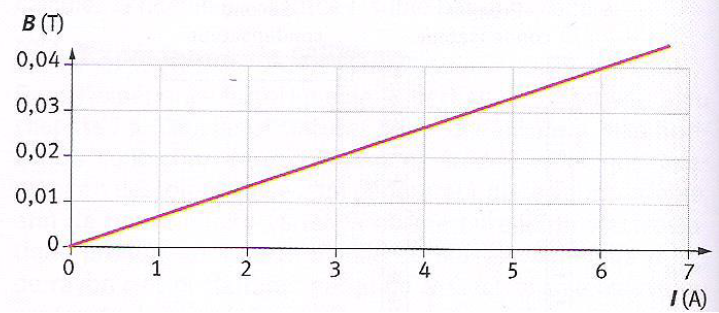
\includegraphics[width=0.5\columnwidth]{images/Exo9_Champ_Magnetique}
\end{center}
%\caption{\label{fig:Logo Objectif Prépas}
\end{figure}

\vspace{0.3cm}

Une sonde permet de mesurer la norme du champ magnétique, notée B, lorsque le solénoïde est parcouru par un courant d'intensité $I$. Le graphe représentant les variations de $B$ en fonction de $I$ est proposé ci-contre. Dans les unités du système international, $B = 4\pi.10^{-7} \times \frac{N}{L} I$, où $N$ est le nombre de spires du solénoïde et $L$ sa longueur exprimée en mètre.

\newpage

\item \begin{enumerate}[label=(\alph*)]
\item Quel est le nom de l'unité correspondant à la lettre $T$ ?
\item Déduire $N$ du graphique sachant que la longueur du solénoïde est $L = 0,30\text{ }\meter$.
\end{enumerate}

\vspace{0.3cm}

En annexe se trouve une coupe de la Terre avec les lignes de champ magnétique terrestre. A Paris, le champ magnétique terrestre plonge vers le sol. L'angle entre le plan horizontal et le vecteur champ magnétique est d'environ $65\text{ }\degree$. La composante horizontale du champ magnétique terrestre a pour valeur $B_{Th} = 0,20 . 10^{-4}\text{ }\tesla$.

\item \begin{enumerate}[label=(\alph*)]
\item Tracer, sur la coupe de la Terre (en annexe), la verticale et l'horizontale à Paris.
\item Tracer le vecteur champ magnétique à Paris.
\item A l'aide d'un rapporteur, vérifier l'angle de $65\text{ }\degree$ annoncé.
\item Quelle est la direction et le sens du vecteur champ magnétique au pôle Nord ? Au pôle Sud ?
\item Selon quelle direction va s'orienter une boussole à l'un ou l'autre des pôles ?
\item Quels sont la direction et le sens du vecteur champ magnétique au niveau de l'équateur ?
\item Comparé à $B_{Th}$, la norme du champ magnétique créé par le solénoïde pour une intensité $I=3\text{ }\ampere$. Est-elle environ: $10$ fois plus intense, $1000$ fois plus intense, $10$ fois moins intense, ou $1000$ fois moins intense.
\end{enumerate}
\end{enumerate}

\vspace{0.3cm}

\begin{minipage}[c]{.46\linewidth}
\begin{center}
\textbf{Schéma du solénoïde}
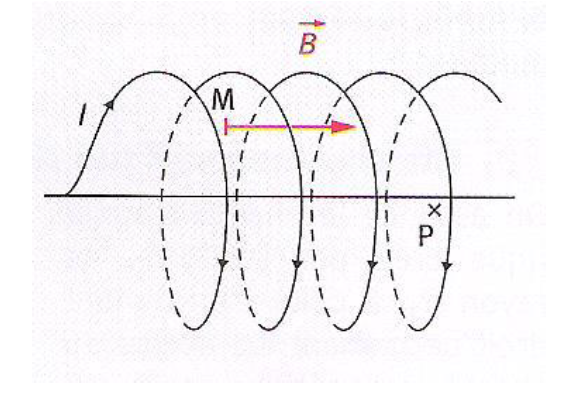
\includegraphics[width=0.75\columnwidth]{images/Exo9_Solenoide}
\end{center}
\end{minipage}
\begin{minipage}[c]{.46\linewidth}
\begin{center}
\textbf{Schéma coupe de la Terre}
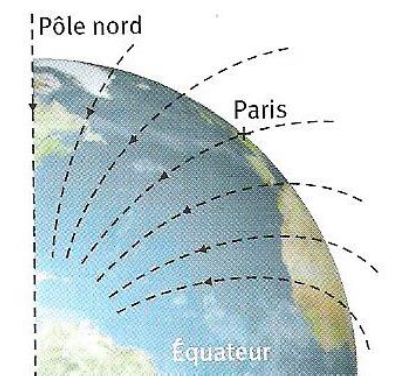
\includegraphics[width=0.5\columnwidth]{images/Exo9_Schema_Coupe_Terre}
\end{center}
\end{minipage}

\vspace{0.3cm}

%%%%%%%%%%%%%%%%%%%%%%%%%%%%%%%%%%%%%%%%%%%%%%%%%%%%%%%%%%%%%%%%%%%%%%%%%%%%%%%%%%%%%%%%%
\exo \textbf{Réactions d'oxydoréduction}

\vspace{0.3cm}

On fait réagir une masse $m=1,0\text{ }\gram$ de fer en poudre avec un volume $V=20\text{ }\milli\liter$ d'une solution de chlorure
d'hydrogène (\chemform{H^{+}};\chemform{Cl^{-}}) de concentration $C=2,0\text{ }\mole.\liter^{-1}$. On observe un dégagement gazeux et l'apparition
d'une coloration vert pâle dans la solution.\newline
Le gaz est identifié en présentant une allumette enflammée. Il se produit une légère explosion (aboiement). Les ions responsables de la coloration sont identifiés en faisant réagir avec un peu de solution, une solution
d'hydroxyde de sodium. Lorsqu'on introduit la solution d'hydroxyde de sodium dans la solution on obtient un précipité vert.

\vspace{0.3cm}

\textbf{Tests caractéristiques de quelques ions}

%\vspace{0.3cm}

\begin{center}
\begin{tabular}{|c|c|c|c|}
\hline
ion testé & couleur solution & formule du réactif: ion réagissant & couleur/formule précipité \\
\hline
\chemform{Cu^{2+}} & bleue & \chemform{Na^{+}+HO^{-}}, ion hydroxyde \chemform{H0^{-}} & précipité bleu, \chemform{Cu(OH)_{2}} \\
\hline
\chemform{Fe^{2+}} & vert & \chemform{Na^{+}+HO^{-}}, ion hydroxyde \chemform{H0^{-}} & précipité vert, \chemform{Fe(OH)_{2}} \\
\hline
\chemform{Fe^{3+}} & rouge & \chemform{Na^{+}+HO^{-}}, ion hydroxyde \chemform{H0^{-}} & précipité rouille, \chemform{Fe(OH)_{3}} \\
\hline
\chemform{Zn^{2+}} & rouge & \chemform{Na^{+}+HO^{-}}, ion hydroxyde \chemform{H0^{-}} & précipité blanc, \chemform{Zn(OH)_{2}} \\
\hline
\chemform{Ag^{+}} & incolore & \chemform{Na^{+}+Cl^{-}}, ion chlorure \chemform{Cl^{-}} & précipité blanc, noircit à la lumière, \chemform{Ag(Cl)} \\
\hline
\end{tabular}
\end{center}

%\vspace{0.3cm}

\newpage

\textbf{Tests d'identification de quelques gaz}

%\vspace{0.3cm}

\begin{figure}[h]
\begin{center}
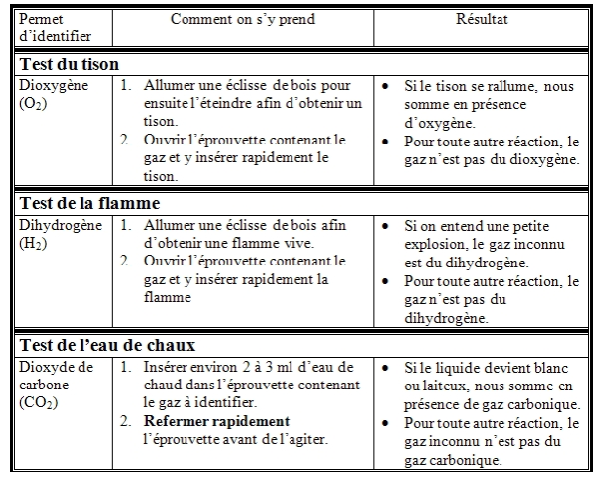
\includegraphics[width=0.75\columnwidth]{images/Exo10_Test_Identification_Gaz}
\end{center}
%\caption{\label{fig:Logo Objectif Prépas}
\end{figure}

\begin{enumerate}
\item Donner, en justifiant les réactifs et les produits de la réaction.
\item Donner, en justifiant vos réponses, les couples oxydant réducteurs mis en jeu dans cette réaction.
\item  Donner les demi-équations associées à ces couples.
\item En déduire l'équation de la réaction qui a lieu.
\item Déterminer les quantités de matière initiales des réactifs.
\item Dresser le tableau d'avancement de la réaction.
\item Déterminer l'avancement maximal de la réaction $x_{max}$.
\item En déduire le volume de gaz dégagé en fin de réaction.
\end{enumerate}

\vspace{0.3cm}

\textbf{Données:}

\vspace{0.3cm}

Le volume qu'occupe un gaz est proportionnel à la quantité de matière de gaz selon la relation: $V = n \times V_{m}$, avec $V_{m} = 24,0\text{ }\liter.\mole^{-1}$.

\vspace{0.3cm}

$M(Fe) = 55,8\text{ }\gram.\mole^{-1}$

\newpage

%%%%%%%%%%%%%%%%%%%%%%%%%%%%%%%%%%%%%%%%%%%%%%%
%%%%%%%%%%%%%%%%%%%%%%%%%%%%%%%%%%%%%%%%%%%%%%%
\maketitle{Ondes}
%%%%%%%%%%%%%%%%%%%%%%%%%%%%%%%%%%%%%%%%%%%%%%%
%%%%%%%%%%%%%%%%%%%%%%%%%%%%%%%%%%%%%%%%%%%%%%%

%%%%%%%%%%%%%%%%%%%%%%%%%%%%%%%%%%%%%%%%%%%%%%%%%%%%%%%%%%%%%%%%%%%%%%%%%%%%%%%%%%%%%%%%%
\exo \textbf{Principe de l'échographie}

\vspace{0.3cm}

\textbf{Document $1$ : principe de l'échographie}

\vspace{0.3cm}

La sonde de l'échographe émet des ultrasons et sert aussi de détecteur. Lorsqu'un écho (une onde réfléchie) arrive sur la sonde, il créé sur les transducteurs une légère variation de tension. Les salves durent seulement environ deux microsecondes et sont envoyées environ toutes les millisecondes, ce qui laisse le temps à l'écho de revenir et d'être détecté ; le son parcourt environ $1,5\text{ }\centi\meter$ en $10$ microsecondes dans les tissus mous.\newline
Différentes fréquences sont utilisées en fonction de la zone à visualiser. Les ondes de basse fréquence sont moins atténuées et pénètrent donc plus profondément dans les milieux. Par exemple à $5\text{ }\mega\hertz$, on peut explorer des zones jusqu'à $12\text{ }\centi\meter$ de profondeur, alors qu'à $10\text{ }\mega\hertz$ on atteint seulement $6\text{ }\centi\meter$. Pourquoi alors ne pas se cantonner aux ondes de plus basses fréquences ? Parce que la précision dépend aussi de la fréquence, mais en sens inverse, c'est-à-dire que la résolution est d'autant meilleure que la fréquence est élevée (elle vaut par exemple $0,30\text{ }\milli\meter$ à $5\text{ }\mega\hertz$, mais atteint $0.15\text{ }\milli\meter$ à $10\text{ }\mega\hertz$).

\vspace{0.3cm}

D'après C. Ray, J-C Poizat, "La physique par les objets quotidiens".

\vspace{0.3cm}

\begin{minipage}[c]{.45\linewidth}
\begin{center}
\textbf{Document $2$ : schéma du principe de l'échogramme du cerveau}
%\vspace{0.3cm}
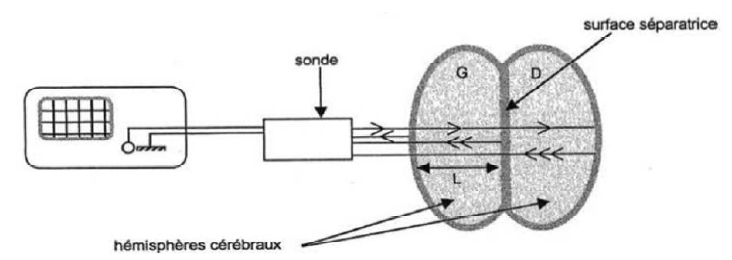
\includegraphics[width=\columnwidth]{images/Exo1_Ondes_Schema_Echogramme_Cerveau}
\end{center}
\end{minipage}
\begin{minipage}[c]{.45\linewidth}
\begin{center}
\textbf{Image d'échographie}\newline
%\vspace{0.3cm}
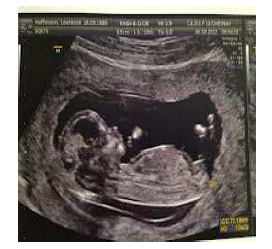
\includegraphics[width=0.45\columnwidth]{images/Exo1_Ondes_Echographie}
\end{center}
\end{minipage}

\vspace{0.3cm}

\textbf{Document $3$ : oscillogramme obtenu lors de l'échogramme du cerveau}

\vspace{0.3cm}

L'oscillogramme obtenu sur un patient permet de tracer l'échogramme ci-dessous: les tensions électriques étant redressées, seule la partie positive de celles-ci est envoyée sur l'oscilloscope.

\begin{figure}[h]
\begin{center}
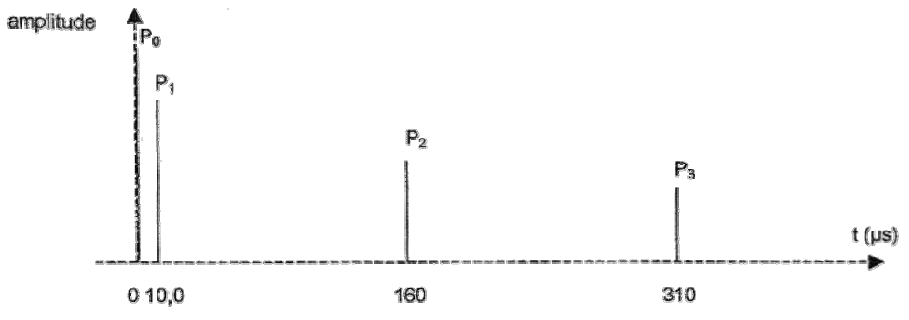
\includegraphics[width=0.75\columnwidth]{images/Exo1_Ondes_Oscillogramme_Echo_Cerveau}
\end{center}
%\caption{\label{fig:Logo Objectif Prépas}
\end{figure}

\begin{enumerate}
\item Que vaut la célérité $v$ des ondes se propageant dans les tissus mous ?
\item Si la fréquence $f$ de l'onde augmente, comment évolue la profondeur $L$ de la zone sondée ? Justifier.
\item Sachant que la précision est d'autant meilleure que la résolution est faible, indiquer quelle onde il semble préférable d'utiliser pour effectuer des échographies.
\item Calculer la période et la longueur d'onde en $\milli\meter$ pour des fréquences $f_{1} = 5,0\text{ }\mega\hertz$ et $f_{2} = 10\text{ }\mega\hertz$.
\item Quel semble être le rapport entre longueur d'onde et résolution ?
\newpage
\item Quelle relation permet de calculer la distance $d$ séparant la sonde du bord d'un organe, en fonction du temps écoulé $\Delta t$ entre l'émission de l'onde et sa réception par le détecteur et la célérité $v$ de l'onde ?
$P_{0}$ correspond à l'émission de l'impulsion à $t = 0\text{ }second$.
\item Déterminer la durée $\Delta t_{g}$ du parcours de l'onde ultrasonore dans l'hémisphère gauche. Même question
pour $\Delta t_{d}$ l'hémisphère droit.
\item En déduire la largeur $L_{g}$ et $L_{d}$ de chaque hémisphère gauche et droit ? Conclure.
\end{enumerate}

\vspace{0.3cm}

%%%%%%%%%%%%%%%%%%%%%%%%%%%%%%%%%%%%%%%%%%%%%%%%%%%%%%%%%%%%%%%%%%%%%%%%%%%%%%%%%%%%%%%%%
\exo \textbf{Accorder une guitare}

\vspace{0.3cm}

Lorsque deux notes ont des fréquences proches, leur mélange produit un son dont l'intensité varie au cours du temps. Ce phénomène, appelé "battement", peut être utilisé pour accorder la $5^{e}$ corde d'une guitare à l'aide d'un diapason. Cette corde émet normalement un La dont la fréquence du fondamental est $110\text{ }\hertz$. On considère que le son émis par un diapason est pur.

\begin{figure}[h]
\begin{center}
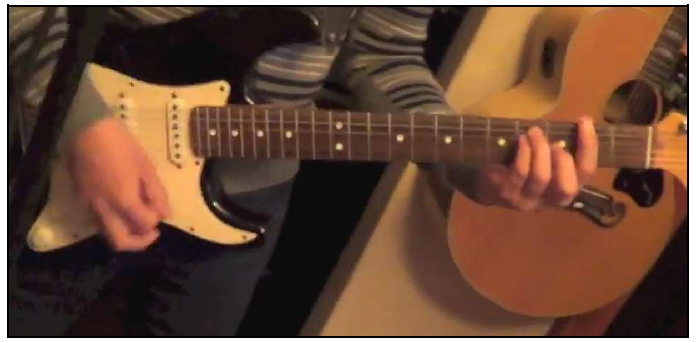
\includegraphics[width=0.75\columnwidth]{images/Exo2_Ondes_Guitare}
\end{center}
%\caption{\label{fig:Logo Objectif Prépas}
\end{figure}

\vspace{0.3cm}

Lya souhaite vérifier la rigueur de cette méthode. Elle enregistre simultanément les sons émis par sa guitare et un diapason et obtient l'oscillogramme ci-dessous à partir duquel elle trace le spectre correspondant.

\begin{figure}[h]
\begin{center}
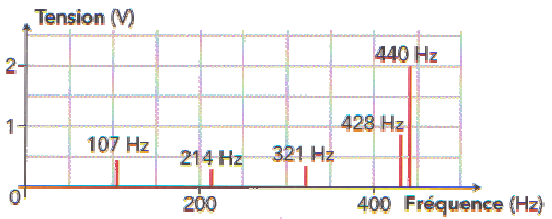
\includegraphics[width=0.5\columnwidth]{images/Exo2_Ondes_Oscillogramme}
\end{center}
%\caption{\label{fig:Logo Objectif Prépas}
\end{figure}

\vspace{0.3cm}

\begin{enumerate}
\item D'après le spectre, quelles sont les fréquences du fondamental et des harmoniques de la note émise par la guitare ?
\item Quelle est la fréquence de la note émise par le diapason ?
\item La corde est-elle accordée ? Justifier.
\item Lya modifie la tension de la corde et réalise une nouvelle acquisition dont le spectre est le suivant :

\begin{figure}[h]
\begin{center}
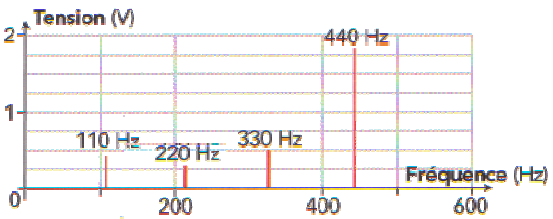
\includegraphics[width=0.5\columnwidth]{images/Exo2_Ondes_Oscillogramme2}
\end{center}
%\caption{\label{fig:Logo Objectif Prépas}
\end{figure}

%\vspace{0.3cm}

\newpage

Régis se trouve à $10\text{ }\meter$ de Lya, qui frappe alors le diapason (sans frapper de corde sur la guitare). L'intensité sonore perçue par le sonomètre de Régis vaut $1,0 . 10^{-10}\text{ }\watt.\meter^{-2}$.

\item Déterminer le niveau sonore $L$ correspondant sachant que $L = 10 \log\left(\frac{I}{I_{0}}\right)$ avec $I_{0} = 1,0 . 10^{-12}\text{ }\watt.\meter^{-2}$.

\item Quelle est la valeur du niveau sonore capté par le sonomètre de Régis si Lya frappe $3$ diapasons identiques en même temps (en supposant qu'elle y arrive) ? Justifier.

\item Combien de diapasons faut-il frapper en même temps pour que le sonomètre de Régis indique une valeur de $30\text{ }\deci\bel$ ? Justifier.

\end{enumerate}

\vspace{0.3cm}

%%%%%%%%%%%%%%%%%%%%%%%%%%%%%%%%%%%%%%%%%%%%%%%%%%%%%%%%%%%%%%%%%%%%%%%%%%%%%%%%%%%%%%%%%
\exo \textbf{Ondes sonores}

\vspace{0.3cm}

\begin{enumerate}

\item \textbf{Généralités sur les ondes sonores}

\begin{enumerate}[label=(\alph*)]
\item A quelle grandeur physique se réfère la notion de hauteur d'une note musicale ?
\item Choisir parmi les valeurs numériques, la valeur moyenne de la vitesse de propagation des ondes sonores dans l'air, à température ambiante :

$$340\text{ }\centi\meter.\second^{-1}\text{; }340\text{ }\meter.\second^{-1}\text{; }340\text{ }\kilo\meter.\second^{-1}$$

\item Même question pour des ondes sonores se propageant dans l'eau:

$$15\text{ }\meter.\second^{-1}\text{; }150\text{ }\meter.\second^{-1}\text{; }1500\text{ }\meter.\second^{-1}$$

\item Construire une échelle de fréquence (qualitative) pour les ondes sonores dans l'air. Situer sur
cette échelle les ondes sonores audibles, les ultrasons, les infrasons, les sons graves et les sons
aigus.

\end{enumerate}

\item \textbf{Enregistrement d'un son}

\vspace{0.3cm}

Un son pur de fréquence $f = 12,5\text{ }\hertz$ est émis devant un microphone, relié à un oscilloscope. L'amplitude du signal envoyé par le microphone à l'oscilloscope est de $0,4\text{ }\volt$. Les réglages de l'oscilloscope sont donnés ci-dessous.

\begin{figure}[h]
\begin{center}
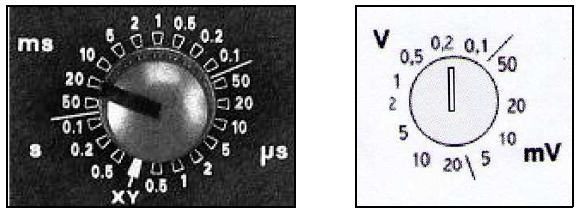
\includegraphics[width=0.5\columnwidth]{images/Exo3_Ondes_Reglages_Oscillo}
\end{center}
%\caption{\label{fig:Logo Objectif Prépas}
\end{figure}

\vspace{0.3cm}

Représenter l'oscillogramme obtenu sur la figure suivante, en justifiant la démarche et les calculs.

\begin{figure}[h]
\begin{center}
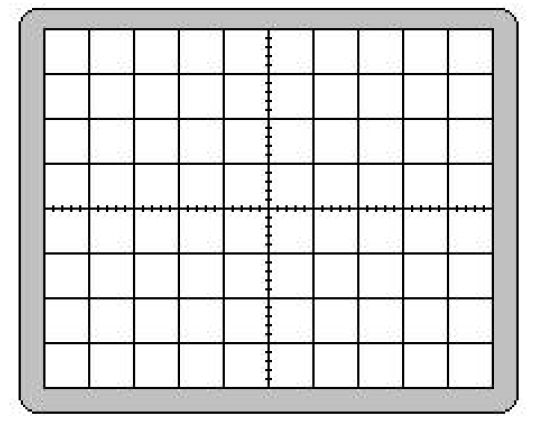
\includegraphics[width=0.5\columnwidth]{images/Exo3_Ondes_Oscillogramme_A_Completer}
\end{center}
%\caption{\label{fig:Logo Objectif Prépas}
\end{figure}

\newpage

\item \textbf{Concert et oreille humaine}

\vspace{0.3cm}

\begin{minipage}[c]{.46\linewidth}
Un ingénieur du son a un rôle primordial
pour la sonorisation des salles, en
particulier lors d'un concert de musique. À
l'aide d'une table de mixage, il règle les
sons qui arrivent depuis les microphones
des musiciens et les renvoie vers les
enceintes de façade et de retour.
L'ingénieur intervient sur quatre qualités
des sons: la hauteur, l'intensité, le timbre
et la durée. Grâce à sa table de mixage, il
convertit facilement un son en un autre. Il
peut notamment modifier un son
correspondant à l'enregistrement $1$ en un
son correspondant à l'enregistrement $2$.
Les différentes représentations d'un son lui
permettent de reconnaître ses caractéristiques (voir enregistrement $3$).
\end{minipage}
\begin{minipage}[c]{.46\linewidth}
\begin{center}
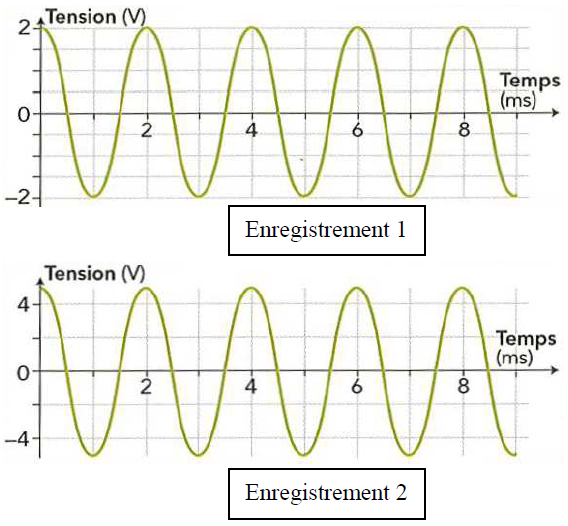
\includegraphics[width=\columnwidth]{images/Exo3_Ondes_Enregistrement_Oscillo}
\end{center}
\end{minipage}

\vspace{0.3cm}

\begin{figure}[!htbp]
\begin{center}
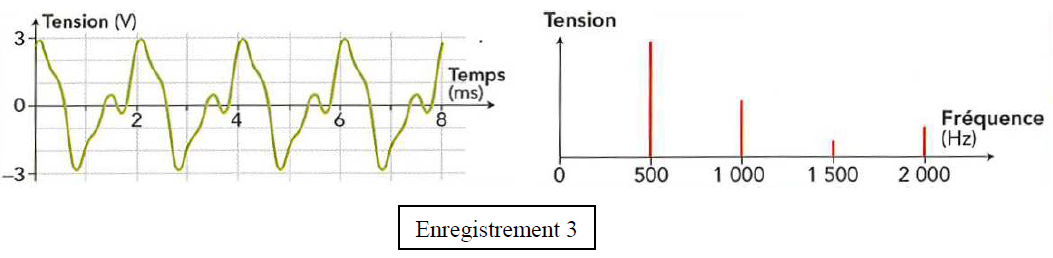
\includegraphics[width=\columnwidth]{images/Exo3_Ondes_Enregistrement_Oscillo3}
\end{center}
%\caption{\label{fig:Logo Objectif Prépas}
\end{figure}

\vspace{0.3cm}

\begin{minipage}[c]{.46\linewidth}
Pour régler le niveau sonore de la salle de
concert, l'ingénieur connait certaines règles.
Par exemple, s'il fait ses réglages pour avoir
un son de $98\text{ }\deci\bel$ pour des spectateurs situés à $16\text{ }\meter$ d'une enceinte, il sait que l'intensité sonore sera quatre fois plus grande pour les spectateurs situés à $8\text{ }\meter$ de l'enceinte. Il sait aussi que l'intensité sonore est doublée s'il place côte à côte deux enceintes identiques. Pour ces réglages l'ingénieur doit tenir compte des seuils de risque, de danger et de douleur. En effet l'exposition à un niveau sonore trop élevé peut provoquer des acouphènes. L'acouphène est un bourdonnement ou sifflement parasite qu'une personne entend
sans que ce bruit existe réellement.
\end{minipage}
\begin{minipage}[c]{.46\linewidth}
\begin{center}
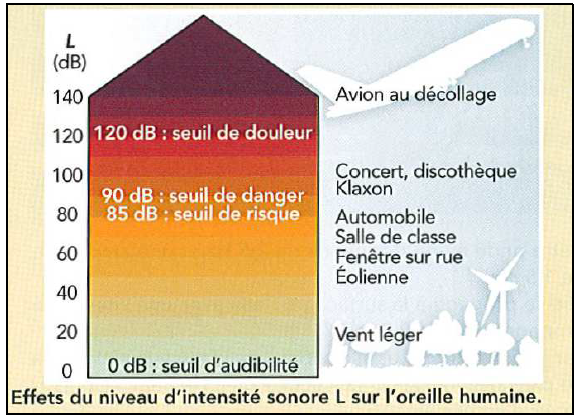
\includegraphics[width=\columnwidth]{images/Exo3_Ondes_Intensite_Sonore_Oreille_Humaine}
\end{center}
\end{minipage}

\vspace{0.3cm}

\begin{enumerate}[label=(\alph*)]
\item Déterminer la fréquence du son correspondant à l'enregistrement $1$.
\item Quelle modification a effectué l'ingénieur du son pour obtenir l'enregistrement $2$ ?
\item En utilisant l'analyse spectrale, montrer que la fréquence du son émis lors de l'enregistrement $3$ est identique à celle des enregistrements $1$ et $2$.
\item Quelle différence présente le son de l'enregistrement $3$ par rapport aux enregistrements $1$ et $2$ ?
\item Quel paramètre du son est ainsi mis en évidence ?
\item Montrer que, pour l'exemple utilisé dans le texte, l'intensité $I_{1}$ du son à $16$ mètres de l'enceinte vaut $I_{1} = 6,3 . 10^{-3}\text{ }\watt.\meter^{-2}$.
\item Si l'ingénieur place $10$ enceintes identiques côte à côte sur scène, déterminer le niveau d'intensité sonore $L_{2}$ à $16$ \meter.
\item On est ici toujours en présence des $10$
enceintes. Sachant que le niveau d'intensité
sonore augmente de $6,0\text{ }\deci\bel$ chaque fois que l'on divise la distance par deux, déterminer à partir de quelle distance des enceintes le son
devient douloureux.
\end{enumerate}

\end{enumerate}

\vspace{0.3cm}

\textbf{Données: }$I_{0} = 10^{-12}\text{ }\watt.\meter^{-2}$

\vspace{0.3cm}

%%%%%%%%%%%%%%%%%%%%%%%%%%%%%%%%%%%%%%%%%%%%%%%%%%%%%%%%%%%%%%%%%%%%%%%%%%%%%%%%%%%%%%%%%
\exo \textbf{Surfer sur la vague (d'après Bac S $2013$ - Amérique du Nord)}

\vspace{0.3cm}

\textit{La houle est un train de vagues régulier généré par un vent soufflant sur une grande étendue de mer sans obstacle, le fetch. En arrivant près du rivage, sous certaines conditions, la houle déferle au grand
bonheur des surfeurs !}

\vspace{0.3cm}

Les documents utiles à la résolution sont rassemblés à la fin de l'exercice.

\vspace{0.3cm}

\textbf{Donnée: }intensité de la pesanteur: $g = 9,8\text{ }\meter.\second^{-2}$

\begin{enumerate}

\item \textbf{La houle, onde mécanique progressive.}

\begin{enumerate}[label=(\alph*)]
\item Pourquoi peut-on dire que la houle est une onde mécanique progressive ?
\item Il est possible de simuler la houle au laboratoire de physique avec une cuve à ondes en utilisant une lame vibrante qui crée à la surface de l'eau une onde progressive sinusoïdale de fréquence $f = 23\text{ }\hertz$. On réalise une photographie du phénomène observé (document $1$).\newline
Déterminer, en expliquant la méthode utilisée, la vitesse de propagation $v$ de l'onde sinusoïdale générée par le vibreur.
\item Au large de la pointe bretonne, à une profondeur de $3000$ \meter, la houle s'est formée avec une longueur d'onde de $60$ \meter. En utilisant le document $2$, calculer la vitesse de propagation $v_{1}$ de cette houle. En déduire sa période $T$.

\item Arrivée de la houle dans une baie.

\begin{enumerate}
\item Sur la photographie aérienne du document $3$, quel phénomène peut-on observer ? Quelle est la condition nécessaire à son apparition ?
\item Citer un autre type d'onde pour laquelle on peut observer le même phénomène.
\end{enumerate}

\end{enumerate}

\item \textbf{Surfer sur la vague}

\begin{enumerate}[label=(\alph*)]
\item La houle atteint une côte sablonneuse et rentre dans la catégorie des ondes longues.
Calculer la nouvelle vitesse de propagation $v_{2}$ de la houle lorsque la profondeur est égale à $4,0\text{ }\meter$. En déduire
à l'aide du document $4$ sa nouvelle longueur d'onde $\lambda_{2}$. D'après ces calculs, la longueur d'onde de la houle varie-t-elle comme attendu dans le document $4$ ?
\item Un autre phénomène très attendu par les surfeurs, lors des marées importantes est le mascaret. Le mascaret est une onde de marée qui remonte un fleuve. Cette onde se propage à une vitesse $v$ de l'ordre de $5,1\text{ }\meter.\second^{-1}$.\newline
Le passage du mascaret étant observé sur la commune d'Arcins à 17h58, à quelle heure arrivera-t-il à un endroit situé à une distance $d = 13\text{ }\kilo\meter$ en amont du fleuve ?
\end{enumerate}

\end{enumerate}

\begin{figure}[h]
\begin{center}
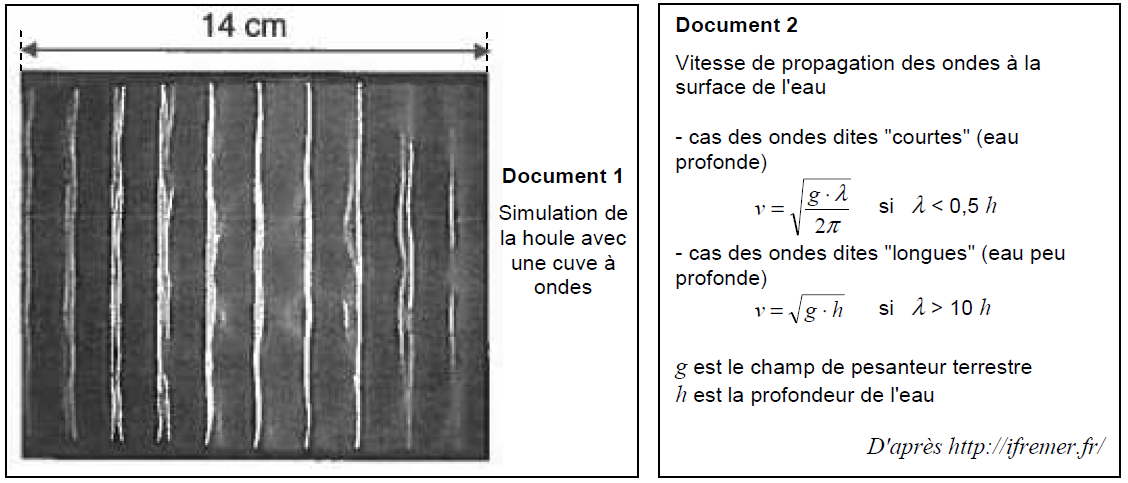
\includegraphics[width=\columnwidth]{images/Exo4_Ondes_Vagues}
\end{center}
%\caption{\label{fig:Logo Objectif Prépas}
\end{figure}

\vspace{0.3cm}

\textbf{Document $3$ : photographie aérienne de l'arrivée de la houle dans une baie.}

\begin{figure}[h]
\begin{center}
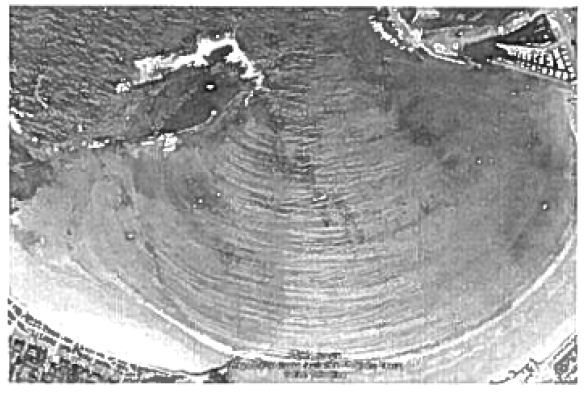
\includegraphics[width=0.5\columnwidth]{images/Exo4_Ondes_Vagues_Doc3}
\end{center}
%\caption{\label{fig:Logo Objectif Prépas}
\end{figure}

%\vspace{0.3cm}

\newpage

\textbf{Document $4$ : déferlement des vagues sur la côte.}

\vspace{0.3cm}

En arrivant près de la côte, la houle atteint des eaux peu profondes. Dès que la profondeur est inférieure à la moitié de la longueur d'onde, les particules d'eau sont freinées par frottement avec le sol. La houle est alors ralentie et sa longueur d'onde diminue. Ces modifications des caractéristiques de l'onde s'accompagnent d'une augmentation d'amplitude. La période est la seule propriété de l'onde qui ne change pas à l'approche de la côte.
Ainsi en arrivant près du rivage, la vitesse des particules sur la crête est plus importante que celle des particules
dans le creux de l'onde, et lorsque la crête n'est plus en équilibre, la vague déferle. (\textit{D'après http://ifremer.fr})

\vspace{0.3cm}

%%%%%%%%%%%%%%%%%%%%%%%%%%%%%%%%%%%%%%%%%%%%%%%%%%%%%%%%%%%%%%%%%%%%%%%%%%%%%%%%%%%%%%%%%
\exo \textbf{Etude de sons}

\vspace{0.3cm}

On enregistre à l'aide d'un micro des sons joués par un synthétiseur. Ces sons
sont alors analysés par un ordinateur à l'aide d'un logiciel adapté.

\vspace{0.3cm}

\begin{minipage}[c]{.46\linewidth}
\begin{enumerate}
\item Le son pur
\begin{enumerate}
\item Quel type d'instrument utilise-t-on généralement pour obtenir un son pur ?
\item En utilisant les mots "harmonique", "fondamental" et "spectre" définir ce
qu'est un son pur.
\item Sachant qu'horizontalement une division équivaut à $500$ \micro\second et que
verticalement une division équivaut à $2$ \milli\volt, déterminer la fréquence du son
sur l'enregistrement A. Ce son est-il grave ou aigu ?
\item L'enregistrement B a été obtenu avec les mêmes réglages (même échelle sur le graphe). Quelle propriété du son a ainsi changé entre A et B ?
\end{enumerate}
\item On fait l'acquisition d'un nouveau son noté C avec le synthétiseur, son pour
lequel on effectue une décomposition de Fourier (spectre)
\begin{enumerate}
\item Sans aucun calcul, définir la propriété du son qui diffère clairement entre A et C.
\item Pourquoi peut-on affirmer que le son C est bien une note et non un bruit ?
\item Définir à l'aide du spectre de C la hauteur de la note joué par le synthétiseur.
\item Quel est le rang de l'harmonique absent dans le spectre de C ?
\item Quelle serait la fréquence du fondamental si l'harmonique de rang 5 avait une fréquence de $900$ \hertz ?
\end{enumerate}
\item Un sonomètre indique que le niveau sonore $L$ de la note $C$ est de $76$ \deci\bel. Calculer son intensité sonore $I$. (On rappelle que le seuil d'audibilité vaut $I_{0} = 1,0 . 10^{-12}\text{ }\watt.\meter^{-2}$)
\end{enumerate}
\end{minipage}
\begin{minipage}[c]{.46\linewidth}
\begin{center}
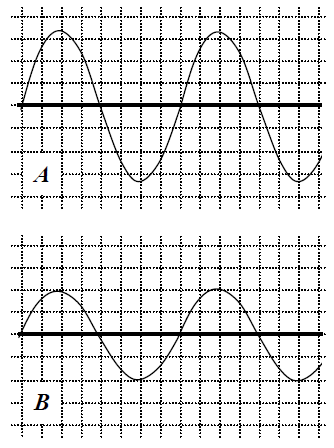
\includegraphics[width=\columnwidth]{images/Exo5_Ondes_Sons}
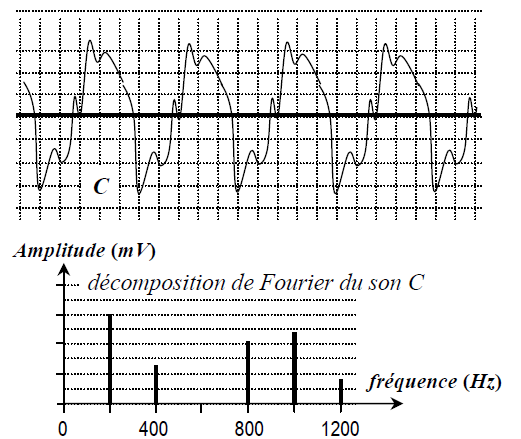
\includegraphics[width=\columnwidth]{images/Exo5_Ondes_Sons_2}
\end{center}
\end{minipage}